\documentclass[xcolor=svgnames,11pt]{beamer}

\usepackage{graphicx}

\usepackage[italian, english]{babel} 
\usepackage[utf8x]{inputenc}

\usepackage{hyperref}
\usepackage{listings}

\usepackage{tabularx}
\usepackage{url}

\usetheme{Goettingen}
\definecolor{android}{RGB}{164,198,57}
\definecolor{myblack}{RGB}{34,34,34}

\usecolortheme[named=myblack]{structure}


\beamertemplateshadingbackground{white!15}{android!15}
\setbeamertemplate{sidebar canvas right}[vertical shading]%
[top=android!100,bottom=white!90]

\setbeamertemplate{blocks}[rounded][shadow=false]
\setbeamercolor{block body}{bg=android!40}
\setbeamercolor{block title}{bg=android!90}

\mode<presentation>{\usebackgroundtemplate{
\includegraphics[height=\paperheight]{back.png}}} 

\setbeamercovered{transparent}

\lstset{
basicstyle=\scriptsize\ttfamily,
keywordstyle=\color{MidnightBlue}\bfseries,
identifierstyle=\color{Black},
commentstyle=\color{Green}\itshape,
stringstyle=\color{Red}\ttfamily,
showstringspaces=false,
numbers=left, numberstyle=\tiny,
stepnumber=1, numbersep=10pt,
tabsize=4,
framexleftmargin=5mm, rulesepcolor=\color{Gray},
frame=tb,
%backgroundcolor=\color{GrigioChiaro},
language={XML},
mathescape=true,
fontadjust=true,
breaklines=true,breakatwhitespace=true,breakautoindent
}

\title{\textbf{Android App Developement: \\ Creare la nostra prima app.}}
\author{Nicola Corti}
\institute{GULP - Gruppo Utenti Linux Pisa \\ Linux Day 2012\\ \medskip  
\includegraphics[height=1.5cm]{ld_logo.png} \hspace{1cm} 
\includegraphics[height=1.5cm]{gulp.png}}
\logo{gulp.png}
\date{25 ottobre 2014}

 
\begin{document}

\begin{frame}
	\titlepage
\end{frame}

\section{Prerequisiti}

\begin{frame}
\begin{center}
\begin{Huge}
{\color{android} Prerequisiti}
\end{Huge}
\end{center}
\end{frame}

\begin{frame}{Prerequisiti}
\textbf{Cosa bisogna sapere per iniziare a programmare per Android?}
\pause
\begin{itemize}
	\item Piccola esperienza con l'ambiente \textbf{Android}
	\pause
	\item Esperienza di programmazione con \textbf{Java}
	\pause
	\item Conoscenza di \textbf{XML}
	\pause
	\item Conoscenza dell'IDE \textbf{Eclipse}
\end{itemize}

\end{frame}

\subsection{Android}
\begin{frame}[fragile]{Android}

\begin{center}

\includegraphics[height=1.5cm]{android.png}
\end{center}
\pause
\textbf{Android} \`e un sistema operativo open per Smartphone e Tablet attualmente sviluppato da Google.\\
\pause
Android \`e basato sul kernel \textbf{Linux}.
\pause
\begin{center}
\visible<4>{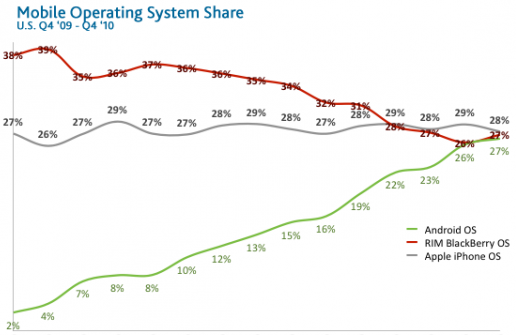
\includegraphics[height=3cm]{chart.png}}
\end{center}
\end{frame}

\subsection{Java}
\begin{frame}{Java}

Java \`e un linguaggio di programmazione \textbf{orientato ad oggetti} ad oggi molto famoso ed utilizzato in svariate piattaforme.
\pause
\begin{center}
\visible<2,3>{
\includegraphics[height=4cm]{java.png}}
\end{center}
\pause
\begin{block}{Imparare Java}
Si pu\`o consultare qualche guida online: \url{ http://www.html.it/guide/guida-java/}
\end{block}

\end{frame}

\subsection{XML}
\begin{frame}{XML}

XML \`e un linguaggio di \textbf{markup}, largamente diffuso nel web per permettere lo scambio di informazioni.\\
\pause
\medskip
Lo utilizzeremo per definire le risorse della nostra applicazione Android.\\
\medskip
\pause
% Immagine XML
\begin{block}{Imparare XML}
Le guide online sono le pi\`u disparate: \url{http://www.html.it/guide/guida-xml-di-base/}
\end{block}

\end{frame}

\begin{frame}[fragile]{XML}

\begin{lstlisting}
<?xml version="1.0" encoding="UTF-8"?>
<utenti>
    <utente>
        <nome>Luca</nome>
        <cognome>Cicci</cognome>
        <indirizzo>Milano</indirizzo>
    </utente>
    <utente>
        <nome>Max</nome>
        <cognome>Rossi</cognome>
        <indirizzo>Roma</indirizzo>
    </utente>
</utenti>
\end{lstlisting}

\end{frame}

\subsection{Eclipse}
\begin{frame}{Eclipse}

Eclipse \`e un \textbf{ambiente di sviluppo integrato}, che ci permetter\`a di gestire facilmente i nostri progetti Android.

\pause
\begin{center}
\visible<2>{
\includegraphics[height=4cm]{luna.png}}
\end{center}

\end{frame}


\section{Scarichiamo l'SDK}

\begin{frame}{Scarichiamo l'SDK}

Per iniziare a programmare abbiamo bisogno di scaricare l'SDK (\emph{Software Development Kit}) di Android.
\pause
\medskip
\begin{block}{Dove scaricare?}
Per scaricare l'SDK andiamo sul sito \url{http://developer.android.com/sdk/index.html} e selezioniamo la versione per il nostro sistema.
\end{block}
\end{frame}

\begin{frame}{Scarichiamo l'SDK}
\begin{center}
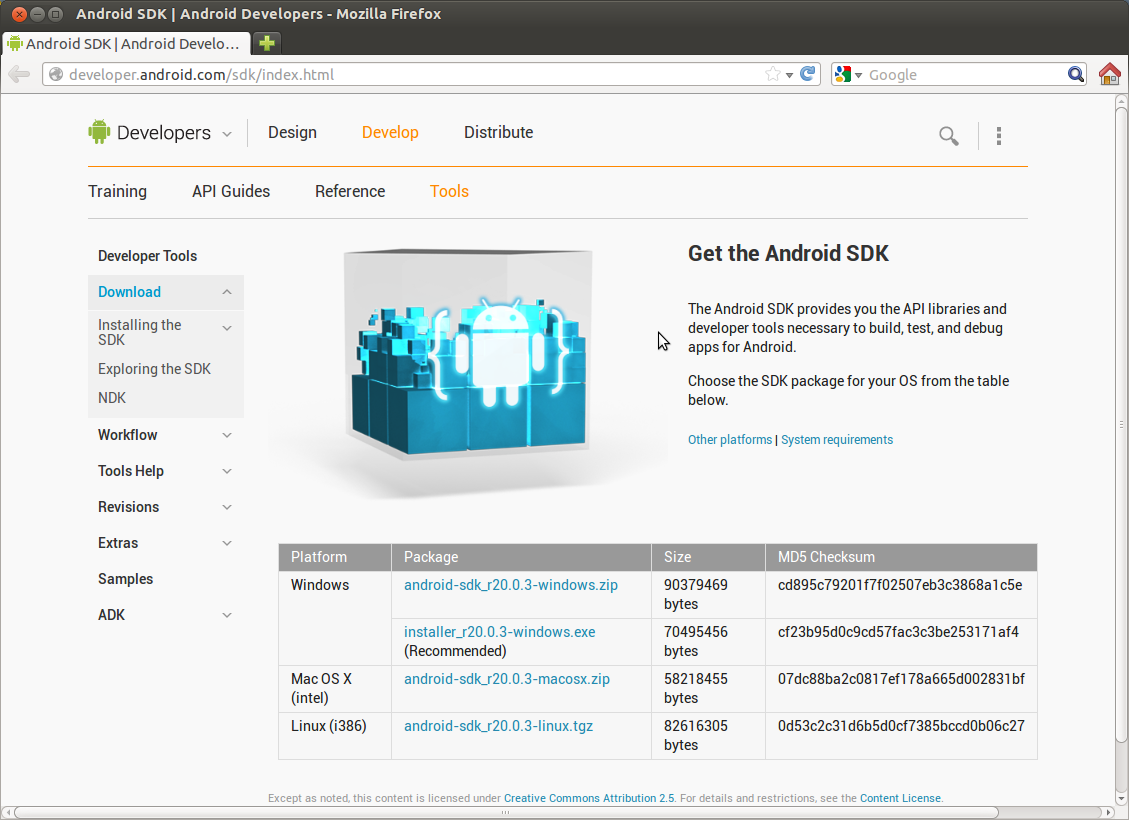
\includegraphics[height=6cm]{sdk.png}
\end{center}
\end{frame}

\subsection{Scarichiamo il plugin ADT}
\begin{frame}{Scarichiamo il plugin ADT}

Scarichiamo il plugin \textbf{ADT} (\emph{Android Development Tool}) per Eclipse.\\
\pause
\medskip
Il plugin \`e necessario per permettere ad Eclipse di gestire progetti Android.
\pause
\medskip
\begin{block}{Repository Google}
Il plugin si puo' scaricare dal repository: \url{http://dl-ssl.google.com/android/eclipse/}
\end{block}
\begin{center}
\visible<4>{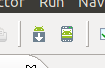
\includegraphics[height=1cm]{crop.png}}
\end{center}
\end{frame}

\begin{frame}{Scarichiamo il plugin ADT}
\begin{center}
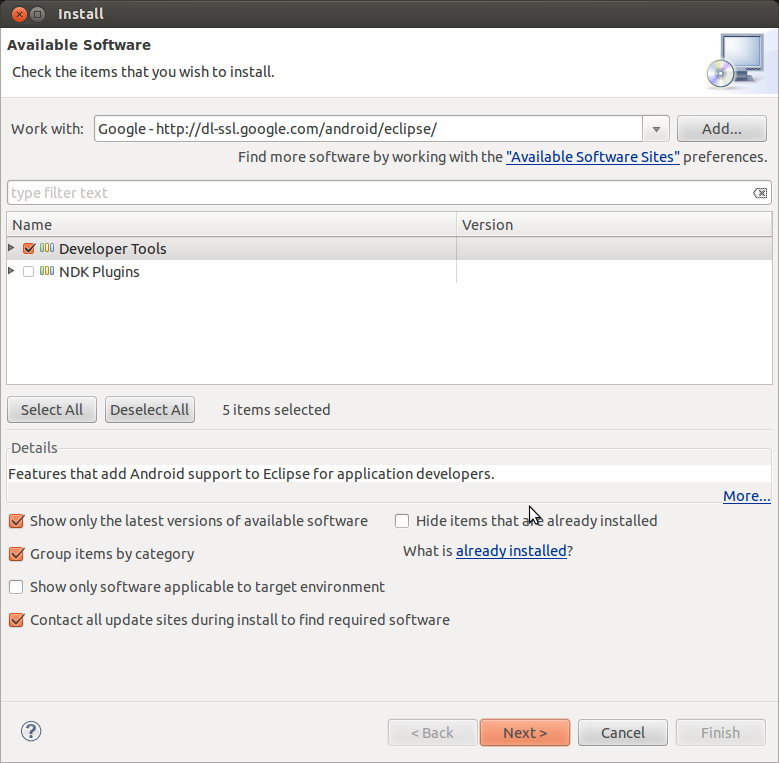
\includegraphics[height=6cm]{adt.png}
\end{center}
\end{frame}

\section{Configurare l'SDK}

\begin{frame}{Configurare l'SDK}
Procediamo a configurare l'SDK per iniziare a programmare
\pause
	\begin{enumerate}
		\item Spacchettiamo l'archivio dell'SDK
		\pause
		\item Eseguiamo il comando: \texttt{tools/android sdk}
		\pause
		\item Scarichiamo i componenti che ci interessano
	\end{enumerate}
\pause
\medskip
\begin{block}{Cosa scarichiamo?}
Scegliamo una versione di Android, verranno scaricati gli \textbf{strumenti per sviluppare}, la \textbf{documentazione}, gli \textbf{esempi}, etc...
\end{block}
\end{frame}

\begin{frame}{Configurare l'SDK}
\begin{center}
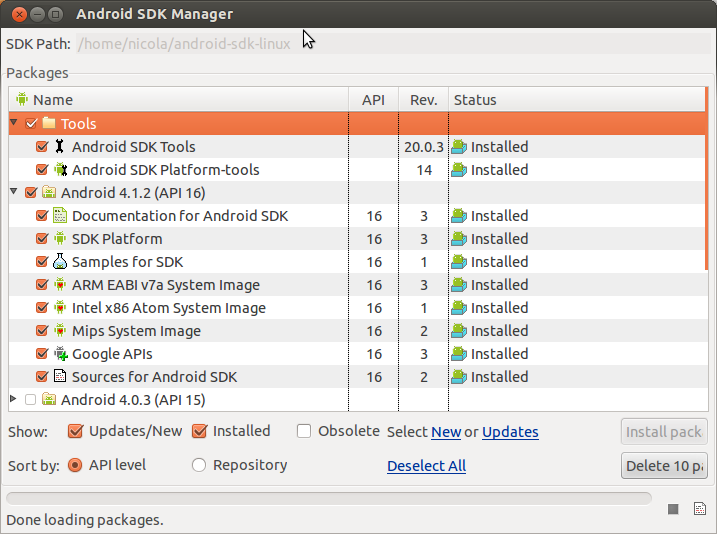
\includegraphics[height=6cm]{manage.png}
\end{center}
\end{frame}

\begin{frame}{Configuriamo l'SDK}
Per chi utilizza Ubuntu a 64 bit \`e necessario scaricare le librerie a 32 bit.
\pause
\medskip
\begin{block}{Shell}
\texttt{sudo dpkg --add-architecture i386}\\
\texttt{sudo apt-get update}\\
\texttt{sudo apt-get install libc6:i386 libncurses5:i386 libstdc++6:i386}
\end{block}
\end{frame}

\subsection{Android Virtual Device}
\begin{frame}{Android Virtual Device}

	Fra i vari strumenti offerti dall'SDK c'\`e \textbf{AVD Manager} (\emph{Android Virtual Device}).\\
	\pause
	\medskip
	Ci permette di creare dei terminali virtuali su cui provare le nostre App.\\
	\pause
	\medskip
	I terminali possono essere utili, ma sono abbastanza \textbf{lenti} e \textbf{poco fluidi}.

\end{frame}
\begin{frame}{Android Virtual Device}

\begin{center}
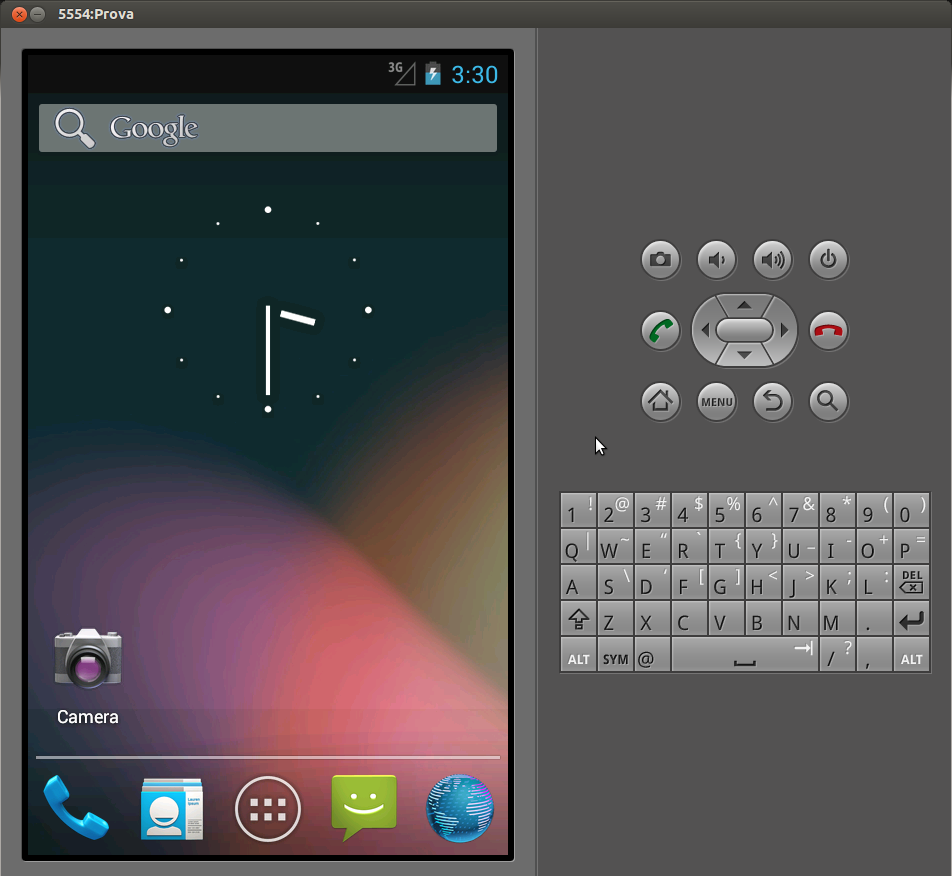
\includegraphics[height=6cm]{avd.png}
\end{center}
\end{frame}

\begin{frame}{Modalit\`a Debug}

	\`E inoltre possibile provare le App su dispositivi Android.\\
	\pause
	\medskip
	L'esecuzione risulta pi\`u veloce e reattiva, inoltre si testa come si comporter\`a l'App su un possibile dispositivo finale.\\
	\pause
	\medskip
	\begin{block}{Modalit\`a Debug}
	Si deve collegare il dispositivo e attivare la \textbf{Modalit\`a Debug} (dentro il men\`u Opzioni per lo Sviluppatore).
	\end{block}	
\end{frame}


\begin{frame}{Modalit\`a Debug}
\begin{center}
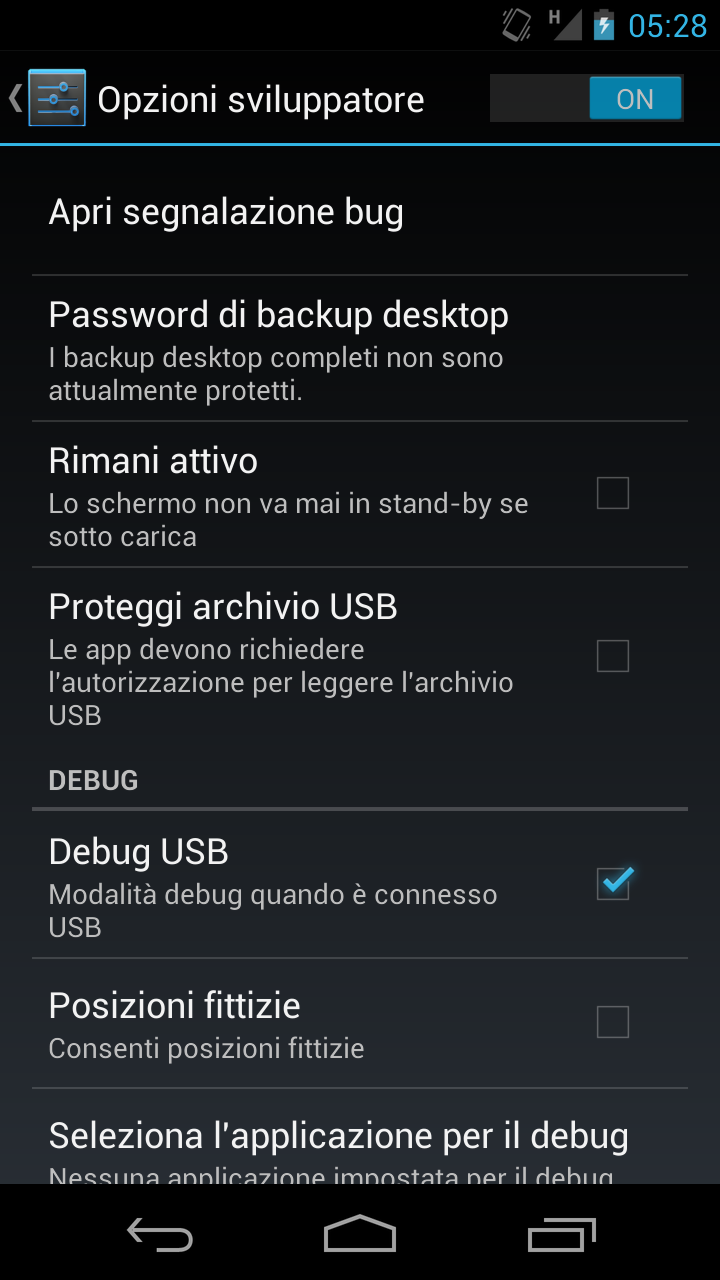
\includegraphics[height=6cm]{debug.png}
\end{center}
\end{frame}

\section{Versioni di Android}

\begin{frame}{Versioni di Android}
L'ecosistema di Android \`e molto eterogeneo. La prima versione di Android \`e uscita nel 2008 e da allora sono uscite molti aggiornamenti del sistema.

\medskip

\begin{center}

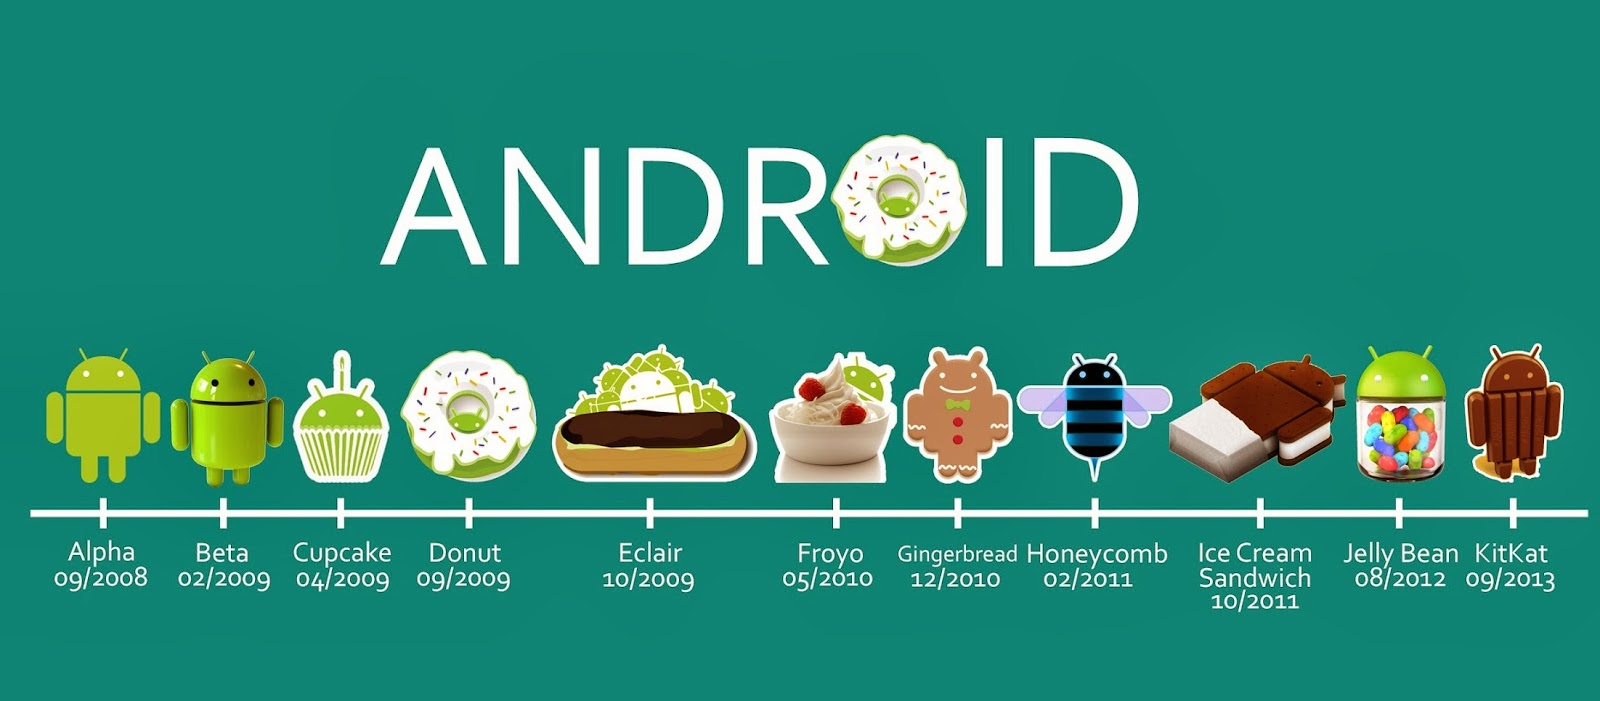
\includegraphics[width=9cm]{versions.jpg}

\end{center}

\pause
\medskip

Quando sviluppiamo dobbiamo tenere in considerazione il fattore \textbf{Versione}.

\end{frame}

%\subsection{API Levels}
\begin{frame}{API Levels}

\medskip

\begin{center}

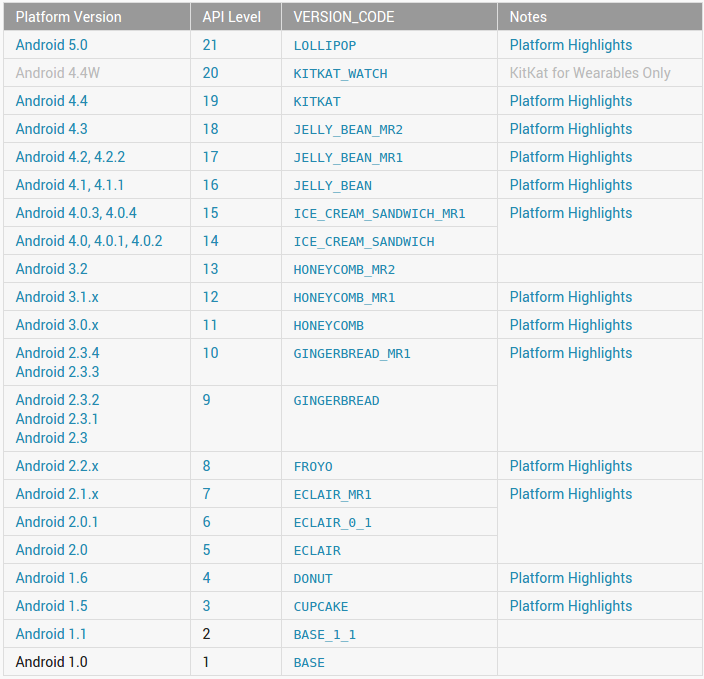
\includegraphics[height=5.5cm]{apilevel.png}

\end{center}

\pause
\medskip

Dobbiamo decidere per quale \textbf{API Level} stiamo sviluppando e fino a quale \textbf{API Level} siamo disposti ad essere retrocompatibili.

\end{frame}

\begin{frame}{API Levels}

\begin{center}
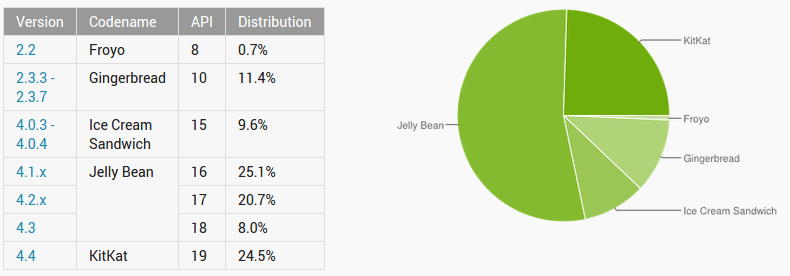
\includegraphics[width=9cm]{dashboard.png}
\end{center}
\end{frame}


\subsection{Dimensioni differenti}
\begin{frame}{Dimensioni differenti}

\begin{center}

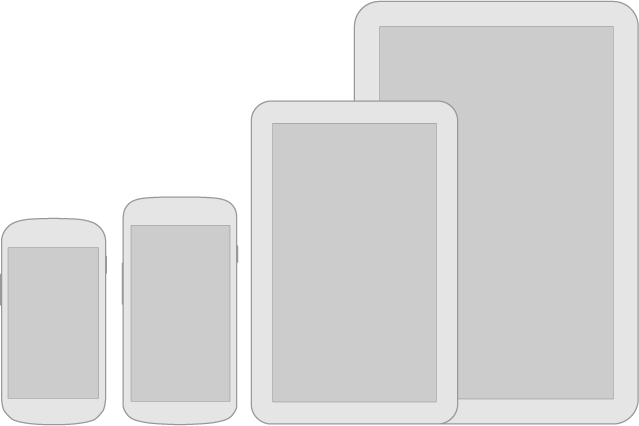
\includegraphics[height=3cm]{devices.png}

\end{center}

\medskip

Android \`e presente su dispositivi che hanno monitor molto differenti fra di loro, partiamo dai \textbf{3 pollici} per arrivare fino ai \textbf{12 pollici}.

\medskip
\pause

\begin{block}{}
\`E essenziale che l'esperienza utente sia gradevole su ogni display dove deve girare l'app; assicurandosi che gli oggetti a schermo si dispongano in modo armonioso. 
\end{block}

\end{frame}

\subsection{AndroidManifest.xml}
\begin{frame}{AndroidManifest.xml}

La definizione globale della nostra app sta nel file \texttt{AndroidManifest.xml}.

\medskip
\pause

All'interno del manifest includeremo \textbf{nome}, \textbf{versione} e \textbf{informazioni generali} dell'app. Tutti i \textbf{moduli} che compongono l'app ed i vari \textbf{permessi straordinari} richiesti dall'applicazione.

\medskip
\pause

\begin{block}{}
Il manifest verr\`a utilizzato dal Play Store per decidere o meno se un'app \`e \textbf{compatibile con il proprio device}.
\end{block}

\end{frame}


\section{Suggerimenti e consigli}

\begin{frame}{Consigli}
\pause
\begin{enumerate}
\item Prima di iniziare assicuratevi di essere in linea con i prerequisiti,
\pause
\item Iniziate con la lettura di un \textbf{libro} che tratti la programmazione Android in modo completo,
\pause
\item \textbf{\emph{Google is your friend...}}
\pause
\item Cercate \textit{snippets} di codice online, copiare il codice non \`e un reato, ma \textbf{prestate attenzione} a cosa includete nella vostra app,
\pause
\item Provate la vostra App su \textbf{devices diversi} ed in \textbf{condizioni differenti} (orientamento, rete, etc...).
\end{enumerate}
\end{frame}

\begin{frame}[fragile]{Design}
Non tralasciate il design della vostra applicazione, pu\`o trasformare un'app \textbf{utile} in un'app \textbf{orrenda}!

\pause
\medskip


\begin{columns}
    \begin{column}{0.3\textwidth}
Argomenti da curare:
\pause
\begin{enumerate}
\item Icone
\pause
\item Loghi
\pause
\item Palette di colori
\pause
\item Bottoni
\pause
\item Animazioni
\pause
\item Font
\end{enumerate}
\end{column}

\begin{column}{0.7\textwidth}
\begin{center}
\visible<2->{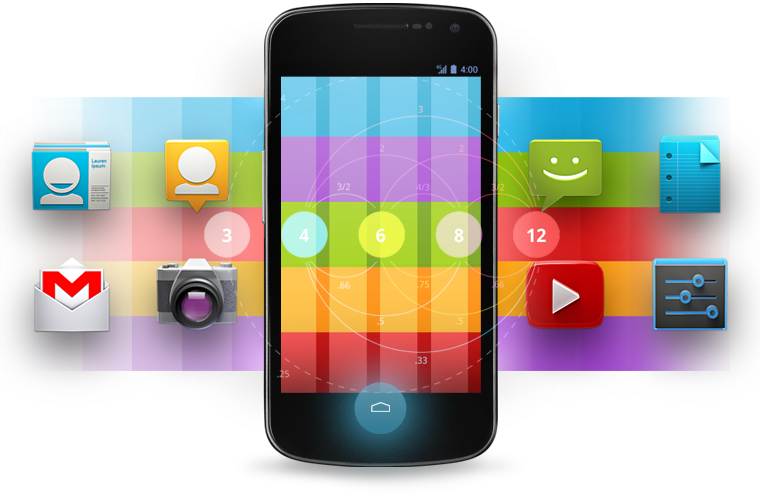
\includegraphics[width=6cm]{palette.png}}
\end{center}
\end{column}
\end{columns}
\end{frame}

\begin{frame}{Material Design}

\begin{center}

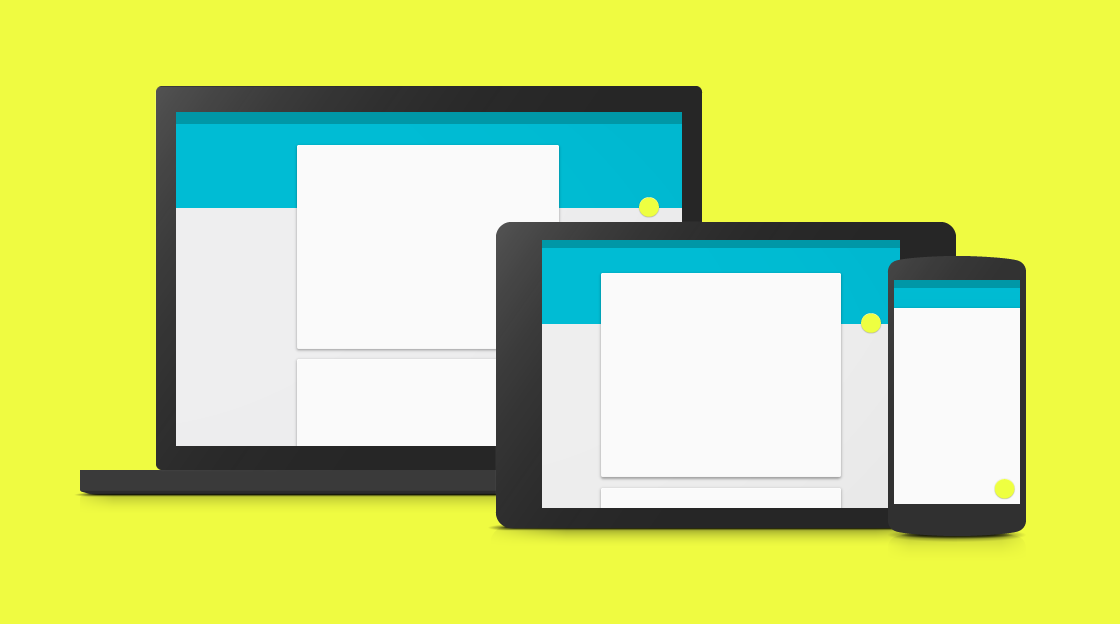
\includegraphics[width=9cm]{material.png}

\bigskip

\url{http://www.google.com/design/spec}

\end{center}

\end{frame}

\section{Conclusione}

\begin{frame}{Guide Online}

\textbf{Online} si trova molto materiale su Android:
\pause
\medskip
\begin{itemize}
\item \small{\url{http://developer.android.com/develop/index.html}}
\pause
\item \url{http://developer.android.com/design/index.html}
\pause
\item \url{http://www.html.it/guide/guida-android/}
\end{itemize}
\end{frame}




\begin{frame}{}

\begin{center}
\begin{Huge}
{\color{android} \textbf{Domande...?}}
\end{Huge}

\vspace{1.5cm}
\begin{small}
Slides realizzate da:\\
\textbf{Nicola Corti - corti.nico [at] gmail [dot] com}\\
\url{http://www.ncorti.it/}

\bigskip

Slides realizzate con \LaTeX\ Beamer.\\
La seguente presentazione \`e rilasciata sotto licenza\\
\begin{footnotesize}	\textbf{Creative Commons - Attributions, Non Commercial, Share-alike}.
\end{footnotesize}
\\
\medskip

\includegraphics[height=0.5cm]{cc.png}

\end{small}
\end{center}
\end{frame}

\end{document}
